\documentclass{article}
\usepackage[utf8]{inputenc}
\usepackage{kotex} 
\usepackage[left=2.5cm,right=2.5cm,top=3cm,bottom=3cm,a4paper]{geometry}

\title{Darknet YOLO API}
\author{이대경, 김한섭, 강일송 }
\date{2017학년도 2학기 오픈소스 Team Project}

\usepackage{natbib}
\usepackage{graphicx}

\begin{document}

\maketitle

\section{You Only Look Once}

\indent YOLO시스템은 최첨단 실시간 물체 감지 시스템이다.
기존의 탐지시스템은 Repurpose classifiers 혹은 Localizers를 사용하여 탐지를 수행하였습니다. 이 방법은 모델의 여러 위치에 격자 이미지를 적용하는 방식이며 격자 중 높은 일치도를 보인 물체를 탐지합니다. 하지만 YOLO는 하나의 신경망을 전체 이미지에 적용하는 완전히 다른 방식을 사용합니다. 이 신경망은 이미지를 여러 영역으로 분할하고 각 영역에 대한 바운딩 영역과 가중치로 사용될 일치 확률을 예측하여 줍니다.

\begin{figure}[h!]
\centering
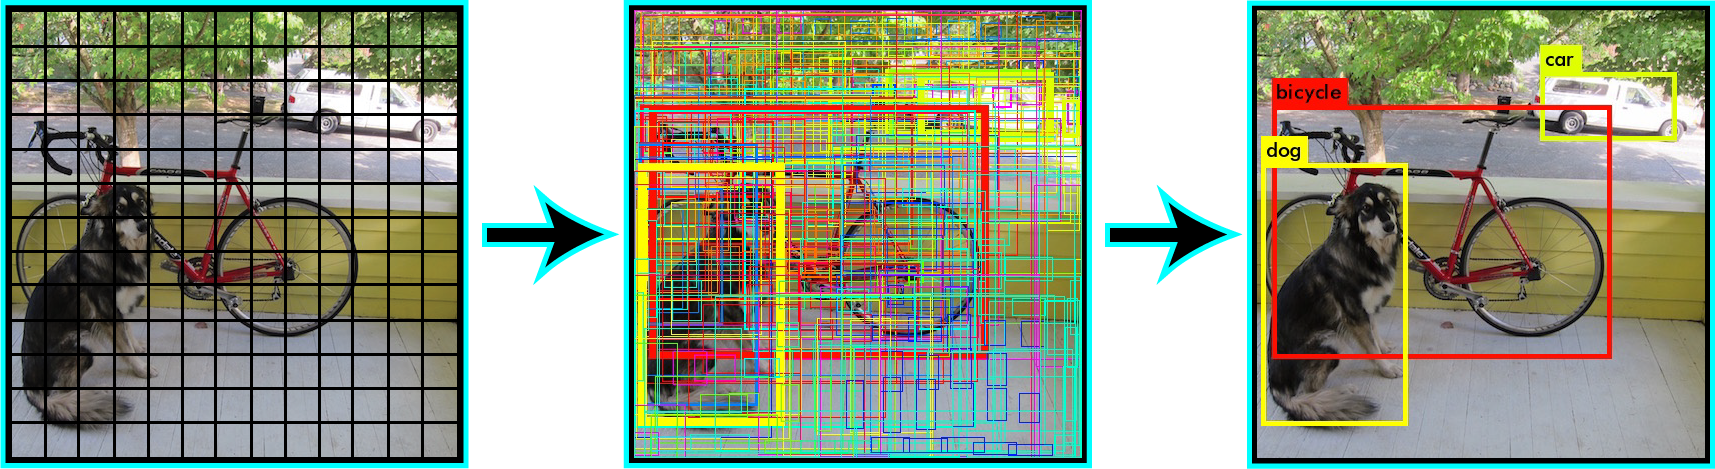
\includegraphics[scale=0.2]{model2.png}
\caption{탐지과정}
\label{fig:univerise}
\end{figure}

YOLO 시스템은 분류 기반의 시스템에 비해 몇 가지 장점을 가지고 있다.
그 중 하나는 테스트 시간 동안 전체 이미지를 보고 예측된 정보를 이미지에 텍스트로 알려줍니다. 또한 수천개의 단일 이미지가 필요한 R-CNN 과는 달리 단일 네트워크만으로 평가하고 예측이 가능합니다. 이로 인해 R-CNN보다는 1000배 이상 빠르며 Fast R-CNN보다는 100배 빠릅니다. 전체 시스템에 대한 자세한 내용은 해당 논문\citep{YOLO9000} 을 참고하시기 바랍니다.


\section{탐지기법 실습}

\indent 사전 훈련 된 모델을 사용하여 YOLO 시스템으로 물체를 탐지 하는 방법을 설명합니다. 
Darknet을 아직 설치 하지 않았다면 먼저 설치 해야합니다. \\
이제부터 아래의 명령어를 실행하시기바랍니다.\\\\
\indent .git clone https://github.com/pjreddie/darknet \\
\indent cd darknet \\
\indent make\\\\
당신에게는 이미 cfg/ 서브디렉토리에 YOLO에 대한 설정 파일이 존재합니다. 
사전 훈련된 가중치를 다운 받고 https://pjreddie.com/media/files/yolo.weights 다음을 실행하시기 바랍니다.

\bibliographystyle{plain}
\bibliography{references}
\end{document}
